\section{Control}
In this project, the quantity to be controlled is the terminal voltage of the generator. The terminal voltage depends on the internally generated voltage \cite{machinery}. Since the rotation speed of the generator is kept constant, the only way to control the internally generated voltage is by controlling the strength of the rotor magnetic field, which, in turn, is dependent on the excitation voltage.
Therefore, the input to our control system is the DC excitation voltage that directly controls the output of the system, which is the terminal voltage.

The control system must be designed for the following scenario: The load on the generator output varies as the connected utilities are turned on and off. When the load changes, the terminal voltage on the generator changes as well \cite{machinery}. For the mostly resistive residential loads, this means that every time a heater or a light gets turned on, there will be a voltage drop in the terminal voltage. Since it is desirable to provide a constant voltage to customers, this voltage drop needs to be compensated quickly by an excitation control system \cite{modern}.

\begin{figure}[h!]
\begin{center}
\includegraphics[scale=0.7]{./img/figure.pdf}
\end{center}
\caption{Feedback Control System for Excitation Control}
\label{fig:sys}
\end{figure}

The control system needs to be a closed-loop feedback control system, with a voltage transducer as a sensor \cite{modern}. In order to minimize the drop in terminal voltage and to speed up the overall response of the generator, a compensator system will have to be designed \cite{modern}. The overall block diagram of the control loop is provided in Figure \ref{fig:sys}.

The voltage transducer measures the terminal voltage and provides feedback to the circuit.  The compensator stabilizes and speeds up the loop and provides the input voltage to the exciter. The exciter creates the magnetic field on the rotor, which determines the terminal voltage.

In order to control the generator at peak performance, a steady-state error of zero was needed, along with a fast settling time and reasonable percent overshoot. Therefore, the choice was made to design a PI compensator. At first, we tried to design it using the recipes learned from the book and in class, but due to the fact that the results of the first test run were too slow, we designed the PI "by hand" using the root-locus method. We chose to place the zero of the compensator far out to the left of the imaginary axis. A zero at -30 provided the desired specifications and led us to victory in the class competition.
Figure \ref{fig:test1} shows the system response for the unsuccessful first test. The compensator used in this test was:
\begin{equation}
G_c(s) = \frac{3.22s + 17}{s}
\end{equation}
Note the slow response time and high overshoot, especially once the inductive load is switched on at t = 175 sec.


\begin{figure}[h!]
\begin{center}
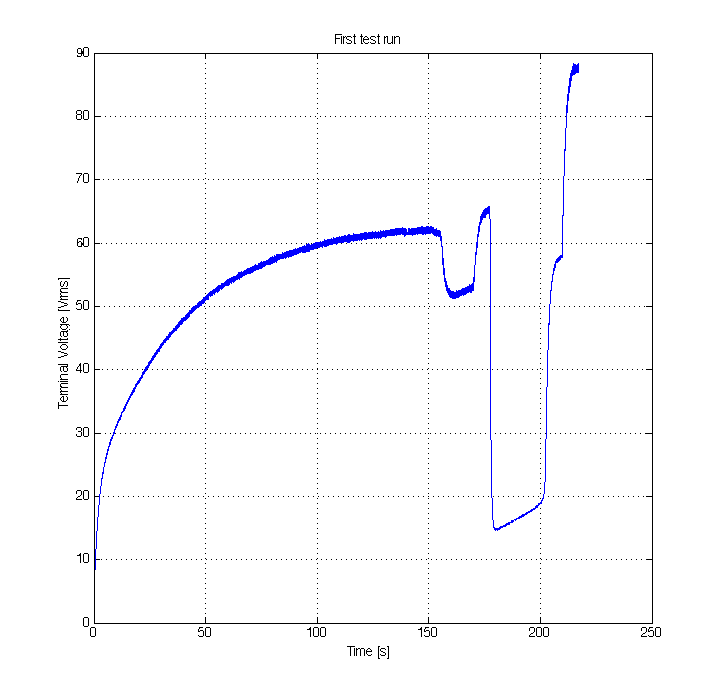
\includegraphics[scale=0.6]{./img/data_first.png}
\end{center}
\caption{Test results for the first test}
\label{fig:test1}
\end{figure}

Figure \ref{fig:final_test} shows the system response for the final test. The compensator used in this test was:
\begin{equation}
G_c(s) = \frac{s + 30}{s}
\end{equation}
Note the fast response time and relatively low overshoot.

\begin{figure}[h!]
\begin{center}
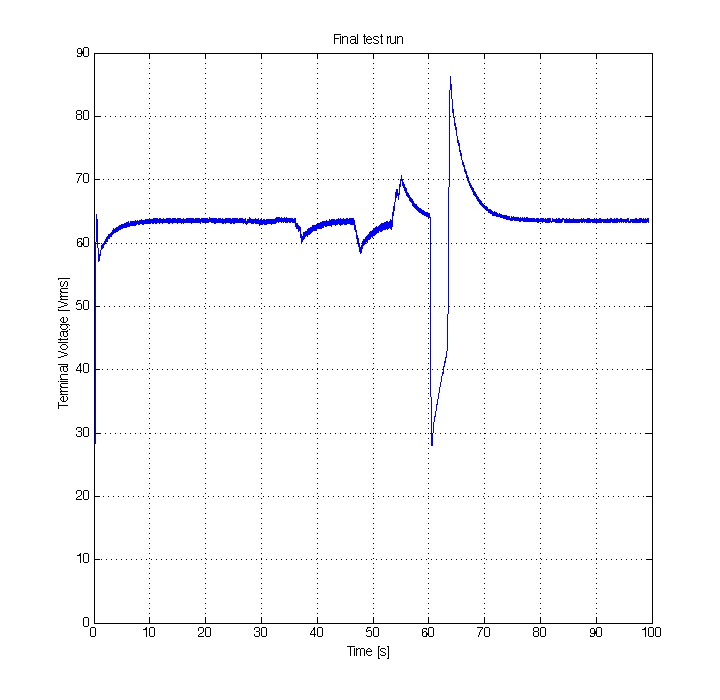
\includegraphics[scale=0.6]{./img/data_final.png}
\end{center}
\caption{Test results for the final test}
\label{fig:final_test}
\end{figure}


